\section{Model predictive control}
\label{cap:mpc_theory}

Model predictive controller (MPC), also known as \textit{receding horizon controller}, is a common technique of controlling unmanned aircraft. Though it is a challenging task to implement it into an embedded hardware, unlike other feedback loop controllers usually used on UAVs, namely PID (proportional-integral-derivative controller) and full-state feedback. The origins of MPC can be found around chemical plants where the time constants of such dynamical processes are relatively high (up to order of hours) thus the computational demand is not so limiting. Also the constraint handling, an inherent property of MPC, is widely used while driving chemical processes. Since then the MPC started to spread on faster systems as the hardware become more powerful. Nowadays it is used to drive systems with sampling in order of milliseconds and tens of hertz loop rate.

The control loop itself is built upon repeatedly optimizing a cost function (usually called \emph{objective function}) with decision variables that represent a desired input action. It is usually a function of all states, desired trajectory and system inputs over a certain time horizon, often called \emph{prediction horizon}. It penalizes (has higher values) the difference between predicted and desired state trajectory. It also penalizes the control action itself which can be interpreted as penalizing the energy used for controlling the system. In other words, the objective function returns a scalar value that quantifies whether the controller drove the system well. Such function can have extrema. Our goal is to find its minimum which follows that the states are changing according to our desired trajectory. The minimum can be local or global, depending on the function itself. It is usually desirable to find the global minimum since that is where the optimal control action is found with respect to the constructed objective function.

There are several classes of continuous optimization problems depending on the type of the objective function and constraints. Problems based on linear or quadratic objective function subjected to linear inequality constraints are commonly . These are historically well studied cases with known methods for solving them. The problem is usually called \textit{Linear Programming} (LP) when optimizing linear function, or \textit{Quadratic Programming} (QP) when optimizing a quadratic function. Since the MPC can be formulated as LP or QP, the control design problem is then basically reduced to solving a QP or LP program and the main focus is left on system modeling and fine-tuning of free parameters of the objective function. The optimization task itself is usually left on dedicated solver that it specialized on the particular function type. In this thesis, we consider only the linear MPC i.e. controlling an LTI system proposed in chapter \ref{cap:system_identification}. The MPC can be formulated as LP or QP, depending on what type of Euclidean norm is used for computing the distance between two states. When using the \mbox{\emph{$\ell^1$}} or \mbox{\emph{$\ell^\infty$}} norm, the formulation leads to a linear program. One can formulate the LP in a way that minimizes the maximal deviation from desired trajectory - this formulation is usually called a \emph{robust MPC} (RMPC). We will focus on the QP formulation (\mbox{\emph{$\ell^2$}} norm, QMPC) since the quadratic penalization can be more expressive the the linear one --- it penalizes large errors more and additionally provides a deadband in the controller.

\subsection{System prediction}

For the purpose of MPC, it is essential to be able to predict a series of system's states $\textbf{\underline{x}} = (\textbf{x}_{[0]}^T, \textbf{x}_{[1]}^T, ..., \textbf{x}_{[M-1]}^T)^T$ based on the initial state $\textbf{x}_{[0]}$ and inputs $\textbf{\underline{u}} = (\textbf{u}_{[0]}^T, \textbf{u}_{[1]}^T, ..., \textbf{u}_{[M-1]}^T)^T$ where $M$ is the length of the prediction horizon. Let us consider a discrete, linear, time-invariant system with $n$ states and $k$ inputs, assuming $\textbf{C} = \textbf{I}$ and $\textbf{D} = \textbf{0}$ (again, assuming there is no direct transfer from the input to the output and the output consist directly of all states).

\begin{equation}
\textbf{x}_{[t+1]} = \textbf{A}\textbf{x}_{[t]} + \textbf{B}\textbf{u}_{[t]}
\label{eq:mpc_lti_system}
\end{equation}

where $\textbf{x}_{[t]} \in \mathbb{R}^{n}$ is the state vector in the sample time $t$, $\textbf{u}_{[t]} \in \mathbb{R}^k$ is the input vector in the sample time $t$, $\textbf{A} \in \mathbb{R}^{n\times n}$ is the system matrix and $\textbf{B} \in \mathbb{R}^{n\times k}$ is the input matrix. First two prediction steps from $\textbf{x}_{[0]}$ can be formulated as

\begin{equation}
\begin{split}
\textbf{x}_{[1]} &= \textbf{A}\textbf{x}_{[0]} + \textbf{B}\textbf{u}_{[0]} \\
\textbf{x}_{[2]} &= \textbf{A}\textbf{x}_{[1]} + \textbf{B}\textbf{u}_{[1]} = \textbf{A}^2\textbf{x}_{[0]} + \textbf{A}\textbf{B}\textbf{u}_{[0]} + \textbf{B}\textbf{u}_{[1]}
\end{split}
\end{equation}

The prediction can be further generalized for any time step as follows

\begin{equation}
\begin{split}
\textbf{x}_{[t+2]} &= \textbf{A}^2\textbf{x}_{[t]} + \textbf{A}\textbf{B}\textbf{u}_{[t]} + \textbf{B}\textbf{u}_{[t+1]}
\end{split}
\end{equation}

The recurrent relation can be used to get the prediction in any future time step.  Moreover, it can be put in the matrix form for all future time steps within the prediction horizon. Matrices denoted in (\ref{eq:prediction_big}) are basic building blocks of QMPC formulation presented on following page.

\begin{equation}
\label{eq:prediction_big}
\underbrace{
\begin{bmatrix}
\textbf{x}_{[1]} \\
\textbf{x}_{[2]} \\
\vdots \\
\textbf{x}_{[M-1]} \\
\end{bmatrix}}_{\textbf{\underline{x}}}
=
\underbrace{
\begin{bmatrix}
\textbf{A} \\
\textbf{A}^2 \\
\vdots \\
\textbf{A}^{M-1} \\
\end{bmatrix}}_{\textbf{\^A}}
\textbf{x}_{[0]}
+
\underbrace{
\begin{bmatrix}
\textbf{B} & \textbf{0} & \textbf{0} & \textbf{0} \\
\textbf{AB} & \textbf{B} & \textbf{0} & \textbf{0} \\
\vdots & \vdots & \ddots & \vdots \\
\textbf{A}^{M-1}\textbf{B} & \textbf{A}^{M-2}\textbf{B} & \hdots & \textbf{B}
\end{bmatrix}
}_{\textbf{\^B}}\underline{\textbf{u}}
\end{equation}

Thus it can be simplified into a form using matrices $\textbf{\^A}$ and $\textbf{\^B}$

\begin{equation}
\textbf{\underline{x}} = \textbf{\^A}\textbf{x}_{[0]} + \textbf{\^B}\textbf{\underline{u}}
\label{eq:prediction_final}
\end{equation}

\subsection{Problem formulation - QMPC}
\label{cap:mpc_formulation}

The objective function for QMPC is formulated as sum of squares of weighted control errors combined with weighted control actions. In our case the weight of the last control error is weighted differently than all the previous errors which is denoted by the second summand in (\ref{eq:qmpc_basic_formulation}). By doing that, we can prioritize the final error in the horizon and force the controller to converge to the desired trajectory.

\begin{equation}
\label{eq:qmpc_basic_formulation}
\mathrm{V}\left(\textbf{\underline{x}}, \textbf{\underline{u}}\right) = \frac{1}{2}\sum_{i=0}^{M-2}\left(\textbf{e}^T_{[i]}\textbf{Q}\textbf{e}_{[i]} + \textbf{u}^T_{[i]}\textbf{P}\textbf{u}_{[i]}\right) + \frac{1}{2}\textbf{e}_{[M-1]}\textbf{S}\textbf{e}_{[M-1]}
\end{equation}

The control error is denoted by $\textbf{e}_{[t]} = \textbf{x}_{[t]} - \textbf{\~x}_{[t]}$ in the time t, $\textbf{Q} \in \mathbb{R}^{n\times n}$ is the state weighting matrix, $\textbf{P} \in \mathbb{R}^{k\times k}$ is the input weighting matrix and $\textbf{S} \in \mathbb{R}^{n \times n}$ is the matrix weighting the final state values. Matrices $\textbf{Q}$, $\textbf{S}$ need to be positive semi-definite ($\textbf{Q}, \textbf{S} \succeq 0$) and matrix $\textbf{P}$ need to be positive definite ($\textbf{P} \succ 0$) to ensure that the function $\mathrm{V}\left(\textbf{\underline{x}}, \textbf{\underline{u}}\right)$ is strictly convex. Moreover, elements of \textbf{\underline{x}} and \textbf{\underline{u}} need to satisfy the system's dynamics (\ref{eq:mpc_lti_system}). Furthermore by inducing (\ref{eq:prediction_final}) into (\ref{eq:qmpc_basic_formulation}) the objective function can be rewritten into matrix form


\begin{equation}
\mathrm{J}(\underline{\textbf{u}}) = \frac{1}{2}\textbf{\underline{u}}^T\underbrace{\left(\textbf{\^B}^T\textbf{\^Q}\textbf{\^B} + \textbf{\^P}\right)}_{\textbf{\^H}}\textbf{\underline{u}} + \textbf{\underline{u}}^T\underbrace{\left(\textbf{\^Q}\textbf{\^B}\right)^T\left(\textbf{\^A}\textbf{x}_{[0]} - \textbf{\underline{\~x}}\right)}_{\textbf{\^c}}
\label{eq:mpc_objective_large}
\end{equation}

where $\textbf{\underline{\~x}} = (\textbf{\underline{\~x}}_{[0]}^T, \textbf{\underline{\~x}}_{[1]}^T, ..., \textbf{\underline{\~x}}_{[M-1]}^T)^T$ is the reference trajectory for all states consisting of a state vector for each step of the prediction horizon, \mbox{$\textbf{\^Q} \in \mathbb{R}^{nM \times nM}$} and $\textbf{\^P} \in \mathbb{R}^{kM\times kM}$ are weighting matrices denoted in (\ref{eq:qmpc_weighting_matrices}). Matrices $\textbf{\^H} \in \mathbb{R}^{kM\times kM}$ and $\textbf{\^c} \in \mathbb{R}^{kM}$ then define the quadratic form. 

\begin{equation}
\label{eq:qmpc_weighting_matrices}
\textbf{\^Q} = \begin{bmatrix}
\textbf{Q} & \textbf{0} & \hdots & \textbf{0} \\
\textbf{0} & \textbf{Q} & \hdots & \vdots \\
\textbf{0} & \hdots & \ddots & \vdots \\
\textbf{0} & \hdots & \hdots & \textbf{S}
\end{bmatrix},
\textbf{\^P} = \begin{bmatrix}
\textbf{P} & \textbf{0} & \hdots & \textbf{0} \\
\textbf{0} & \textbf{P} & \hdots & \vdots \\
\textbf{0} & \hdots & \ddots & \vdots \\
\textbf{0} & \hdots & \hdots & \textbf{P}
\end{bmatrix}.
\end{equation}

Finally the optimization task can be formulated as minimizing the objective function $\mathrm{J}(\textbf{\underline{u}})$ subject to constraints on \textbf{\underline{u}} (which will be discussed in the following paragraphs). This problem is solved repeatedly for new $\textbf{x}_{[0]}$ as the time goes.

\begin{equation}
\label{eq:qmpc_main_quadratic_form}
\begin{aligned}
& \min_{\textbf{\underline{u}} \in \mathbb{R}^{kM}}
& & \mathrm{J}(\underline{\textbf{u}}) = \frac{1}{2}\textbf{\underline{u}}^T\textbf{\^H}\textbf{\underline{u}} + \textbf{\underline{u}}^T\textbf{\^c}\\
& \text{s.t.}
& & \text{constrains on \textbf{u}}
\end{aligned}
\end{equation}

%Before formalizing the linear QMPC, some terms need to be introduced together with their meanings %and ... 
%\begin{table}[h]
%\begin{tabular}{ccl}
%\hline
%& Term & Description \\
%\hline
%$M$ & Prediction horizon length & \parbox[t]{9.65cm} {How many iterations of the LTI system is %computed with in the optimization.} \\
%\hline
%\end{tabular}
%\end{table}

\subsection{Constraints}

When optimizing the quadratic form (\ref{eq:qmpc_main_quadratic_form}) there are usually two types of constraints imposed on the searched solution. The first type is often related to the physical limitations of the controlled system. System's actuators (particularly the physical ones) are not probably designed to accept an arbitrary input signal. For example a servo-motor has a maximum allowed electric current and rotational speed or control surface of an airplane operates within a certain angles of freedom. Let us focus on this type of input constraints defined as \textit{box constraints} i.e. decision variables need to lie within a closed hypercube.

\subsubsection{Input constraints}

Input box constraints allow the controller to find a solution (control actions) that satisfies the input limitations of system's actuators. We can find an analogy in adding a saturation on control outputs of e.g. PID controller. They can be modeled by set of inequalities taking following form

\begin{equation}
\begin{split}
\textbf{b} \leq \textbf{\underline{u}} \leq \textbf{g}
\end{split}
\label{eq:qmpc_input_constraints}
\end{equation}

where $\textbf{b} \in \mathbb{R}^{kM}$ and $\textbf{g} \in \mathbb{R}^{kM}$ are constraint vectors denoting the lower and upper bound on inputs. Such constrained optimization task can be easily solved as it can be seen in chapter \ref{cap:qmpc_unconstrained}. Though it seems more practical to tune parameters of MPC (matrices \textbf{\^Q} and \textbf{\^P}) in a way, that the controller won't naturally produce such control action even when starting from improbable initial conditions. This approach leads to proper control actions anyway so the input constraints can serve as a protection mechanism.

\subsubsection{State constraints}
 
The ability to constrain a particular state's values is one of the main features of the MPC. It can be used to drive the system within some safety region of state variables and to find a control action that won't push the system into unwanted states (sometime irreversibly, e.g. in chemical processes). A convenient example can be found also in a field of unmanned vehicles which can usually operate only within a certain region of velocities and accelerations. By inducing state constraints to the optimization task, it suddenly becomes more difficult to solve. These constraints can be also modeled as a set of linear inequalities using the prediction equation (\ref{eq:prediction_final}). Vectors $\textbf{\underline{v}} \in \mathbb{R}^{nM}$ and $\textbf{\underline{w}} \in \mathbb{R}^{nM}$ denote the lover and upper bounds on states. State constraints create the general linear inequalities of the quadratic programming.
 
\begin{equation}
\textbf{\underline{v}} \leq \textbf{\^A}\textbf{x}_{[0]} + \textbf{\^B}\textbf{\underline{u}} \leq \textbf{\underline{w}}
\label{eq:qmpc_state_constraints}
\end{equation}

\subsubsection{Other constraints}

There are many other types of constraints that can be declared to improve or change the behavior of the system. One particularly useful example is limiting the rate of change of input within the prediction horizon. This leads to smoother input signals and can prevent some stress on actuators of the system. Another possibility is to restrict the monotonicity of a particular state's values over the horizon \citep{rossiter2013mpcpracticalapproach}. This can lead to suppression of overshoots and limiting reactions of unstable zeros (systems with non-minimum phase characteristics) of the system (initially, the system tends to move in the opposite direction than intended). Finally, one can create constraints that force the control signal to lie out of a deadzone of an actuator. Deadzones are inconvenient actuator nonlinearities that can make the control design otherwise very painful.

\subsection{Move blocking -- reducing complexity of MPC}

Up until now, we have considered that each decision variable of the optimization task directly corresponds to a value of input signal in a particular time of the prediction horizon. One could ask whether it is necessary to optimize over the input signal with the same density of signal changes at the beginning as at the end of the prediction horizon. Simulation and experiments show that when coming to the end of the horizon, the optimized input tends to take form of a constant function, assuming the initial condition is sufficiently near to the desired trajectory. Also, supposing the model of the UAV is not perfect and that the control loop (see chapter \ref{cap:qmpc_control_loop}) uses only first few steps of the input signal, there might be an open-loop prediction error too high to payoff for a densely distributed variables. The move blocking technique allows to project a smaller number of variables to cover a longer prediction horizon. The transformation is denoted by following equation

\begin{equation}
\textbf{\underline{u}} = \underbrace{\begin{bmatrix}
\begin{bmatrix}
1\\
\vdots\\
1
\end{bmatrix} & \textbf{0} & \hdots & \textbf{0} \\
\textbf{0} & \begin{bmatrix}
1\\
\vdots\\
1
\end{bmatrix} & \hdots & \textbf{0}\\
\vdots & \vdots & \ddots & \vdots \\
\textbf{0} & \textbf{0} & \hdots & \begin{bmatrix}
1\\
\vdots\\
1
\end{bmatrix}
\end{bmatrix}}_{\textbf{U}}\textbf{\underline{u}}_{r}
\label{eq:moveblocking_example}
\end{equation}

where $\textbf{U} \in \left\lbrace 0, 1 \right\rbrace ^{kM \times kN}$, $N \in \mathbb{N}$ is the number of decision variables and $\textbf{\underline{u}}_{r} \in \mathbb{R}^{kN}$ is the reduced input vector. The MPC task can be then simply modified by creating a new matrix $\textbf{\^B}_{r} = \textbf{\^B}\textbf{U}$ to solve the optimization with and then simply project the variables on the whole horizon. The distribution of variables can vary. One can distribute them evenly or assign a larger portion of them at the beginning of the horizon. This technique can also improve the system's stability by prolonging the horizon when maintaining a similar computational complexity. Although the optimization does not control the system precisely (withing the prediction) the objective function is still in play in every system's step. The chapter \ref{cap:implementation_performance} discuses the particular setting used during the implementation and experiments.

\subsection{Solving QMPC - unconstrained}
\label{cap:qmpc_unconstrained}

The quadratic function in our task is a convex function due to matrices $\textbf{Q}$, $\textbf{S}$ and $\textbf{P}$ which are designed to be positive semi-definite ($\textbf{Q}, \textbf{S} \succeq 0$) and positive definite ($\textbf{P} \succ 0$) respectively. Using this assumption we can find a global minimum by translating it (by a vector $\textbf{\underline{u}}^*$) to the origin and thus changing it to a \textit{quadratic form}. The quadratic form with a semi-definite matrix has a minimum in the origin. The translation can be found by completing the function to the square

\begin{equation}
\begin{split}
\frac{1}{2}\textbf{\underline{u}}^T\textbf{\^H}\textbf{\underline{u}} + \textbf{\underline{u}}^T\textbf{\^c} &= \frac{1}{2}(\textbf{\underline{u}} - \textbf{\underline{u}}^*)^T\textbf{\^H}(\textbf{\underline{u}} - \textbf{\underline{u}}^*)\\
&= \frac{1}{2}\textbf{\underline{u}}^T\textbf{\^H}\textbf{\underline{u}} - \frac{1}{2}\textbf{\underline{u}}^T\textbf{\^H}\textbf{\underline{u}}^* - \frac{1}{2}\textbf{\underline{u}}^{*T}\textbf{\^H}\textbf{\underline{u}} + \frac{1}{2}\textbf{\underline{u}}^{*T}\textbf{\^H}\textbf{\underline{u}}^* \\
&= \frac{1}{2}\textbf{\underline{u}}^T\textbf{\^H}\textbf{\underline{u}} -
\textbf{\underline{u}}^T\textbf{\^H}\textbf{\underline{u}}^* + \frac{1}{2}\textbf{\underline{u}}^{*T}\textbf{\^H}\textbf{\underline{u}}^*
\end{split}
\end{equation}

and by comparing parts of the same degree we get following equations

\begin{equation}
\begin{split}
\textbf{\^c} &= -\textbf{\^H}\textbf{\underline{u}}^* \\
0 &= \frac{1}{2}\textbf{\underline{u}}^{*T}\textbf{\^H}\textbf{\underline{u}}^*
\end{split}
\end{equation}

and finally the solution can be found in a closed-form as $\textbf{\underline{u}}^* = -\textbf{\^H}^{-1}\textbf{\^c}$

\subsection{Solving QMPC - constrained}
\label{cap:qmpc_constrained}

Firstly we will see how to optimally solve QMPC constrained only by the input constraints (\ref{eq:qmpc_input_constraints}). Secondly we will shortly discuss a few QP algorithms for solving QMPC constrained by general linear inequalities (produced by (\ref{eq:qmpc_state_constraints})). Since the work done in this thesis focuses on implementing the first case, only a short survey of QP algorithms is presented.

\subsubsection{QMPC with input constraints}

Input box constrains are a special case of general linear inequalities of QP. Thus they create a convex set of feasible solutions. When the global optimum of a convex quadratic form is not a feasible solution, the actual optimum satisfying the constraints is located on the facet of the convex polytope of the feasible set \citep{boyd2004convex}. One can find it by projecting the unconstrained optimum orthogonally on the feasible set. In the case of box constrains imposed on decision variables this can be done by using $\mathrm{median}$ function. It is possible to project variables independently on each other because box constrains are orthogonal and perpendicular to their corresponding axis.

\begin{equation}
\begin{split}
\label{eq:qmpc_saturating}
\textbf{\underline{\~u}}^*_i \leftarrow \mathrm{median}\left(\textbf{b}_i, \textbf{\underline{u}}^*_i, \textbf{g}_i\right),  \forall i=0,...,kN
\end{split}
\end{equation}

\newcommand{\boundellipse}[3]% center, xdim, ydim
{(#1) ellipse (#2 and #3)
}

One could ask why this process leads to the optimal solution on a feasibility set. A simple proof can be constructed. The figure \ref{fig:qmpc_constrained_analogy} shows an analogous example for two dimensions. It is assumed that the function $\mathrm{J}(\textbf{\underline{u}})$ is convex. When the global optimum $\textbf{\underline{u}}^*$ is found using the closed form solution and it satisfies all constraints, the task is finished. Otherwise there is a constrained optimum $\textbf{\underline{\~u}}^*$ located in the feasibility set which can be found by (\ref{eq:qmpc_saturating}). If there would be another, different, better solution on the feasible set, we could get to it by following facets of the feasibility set polyhedron \citep{boyd2004convex}. That means the step from $\textbf{\underline{\~u}}^*$ would lower the objective value of $\mathrm{J}(\textbf{\underline{u}})$ thus there would be a negative gradient in the direction. But when using (\ref{eq:qmpc_saturating}), every step of projecting variables violating constraints is a step over a positive gradient (as any step from the global optimum of a convex function). This would lead to a claim that there is a local maximum in $\textbf{\underline{\~u}}^*$ which is contradictory to the assumption.

\begin{figure}[h]
\centering
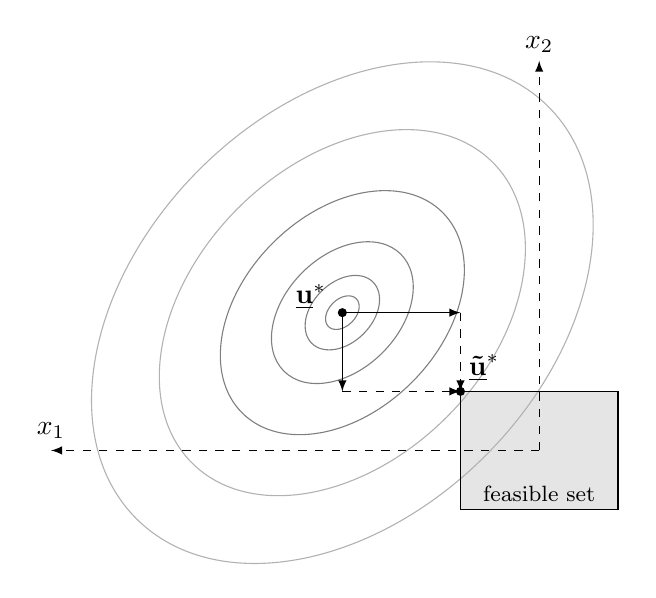
\begin{tikzpicture}

\definecolor{c1}{rgb}{0.7,0.7,0.7}
\definecolor{c2}{rgb}{0.5,0.5,0.5}
\definecolor{podminky}{rgb}{0.9,0.9,0.9}

\fill [podminky] (1.5,-1) rectangle (3.5,-2.5);

\draw[fill] \boundellipse{0,0}{0.05}{0.05};
\draw[color=gray, rotate around={45:(0,0)}] \boundellipse{0,0}{0.25}{0.17};
\draw[color=gray, rotate around={45:(0,0)}] \boundellipse{0,0}{0.55}{0.38};
\draw[color=c2, rotate around={45:(0,0)}] \boundellipse{0,0}{1.05}{0.72};
\draw[color=c2, rotate around={45:(0,0)}] \boundellipse{0,0}{1.8}{1.25};
\draw[color=c1, rotate around={45:(0,0)}] \boundellipse{0,0}{2.7}{2.7/1.44};
\draw[color=c1, rotate around={45:(0,0)}] \boundellipse{0,0}{3.7}{3.7/1.44};

\draw [-latex, dashed] (2.5,-1.75) -- (-3.7,-1.75);
\draw [-latex, dashed] (2.5,-1.75) -- (2.5,3.2);

\draw[fill] \boundellipse{1.5,-1}{0.05}{0.05};
\draw (1.5,-1) -- (3.5,-1) -- (3.5,-2.5) -- (1.5,-2.5) -- (1.5,-1);

\node[] at (-0.4,0.2) {$\textbf{\underline{u}}^*$};
\node[] at (1.8, -0.7) {$\textbf{\underline{\~u}}^*$};
\node[] at (-3.7,-1.5) {$x_1$};
\node[] at (2.5,3.4) {$x_2$};
\node[] at (2.5,-2.3) {\footnotesize feasible set};

\draw[-latex] (0,0) -- (0,-1);
\draw[-latex] (0,0) -- (1.5,0);
\draw[-latex, dashed] (1.5,0) -- (1.5,-1);
\draw[-latex, dashed] (0,-1) -- (1.5,-1);

%\node[] at (0.65,-0.26) {\footnotesize $\frac{\partial\mathrm{J}}{\partial x_1,x_2} > 0$};

%\draw [decorate,decoration={brace,amplitude=10pt},xshift=0pt,yshift=0.1cm]
%(-0.2,0) -- (1.45,-0) node [black,midway,xshift=0pt,yshift=0.6cm] {\footnotesize
%$\frac{\partial\mathrm{J}}{\partial x_1} > 0$};

\end{tikzpicture}
\caption{An illustrative example of 2-dimensional quadratic form with box constraints.}
\label{fig:qmpc_constrained_analogy}
\end{figure}

\subsubsection{QMPC with state constraints}

As it was mentioned previously, the state constraints are the most general of linear inequalities. Solving such quadratic program is a difficult task, compared to the one constrained only by input constraints. The author of \citep{mikulas2013} compares several iterative methods for solving constrained model predictive control. The first one mentioned is the \textbf{Active set method}. It uses the fact that the optimum is attained on the boundary of the feasible set. Throughout the iterations, the algorithm walks along the facets of the convex polytope in a similar way that the \textit{simplex algorithm} for linear programming does. The QP with equality constraints (or unconstrained) is solved every step. The number of iterations depends on the number of constraints active in the optimum.

Another method presented in \citep{mikulas2013} and used in \citep{zometa2012segway} is the \textbf{Fast gradient method}. It is a modification of the classical gradient descend. But instead of moving against the gradient vector, it rather projects it to the feasible set. Its computational demands strongly depend on the projection itself which means it is usually used when only a certain type of constraints is used e.g. box, simplex or Euclidean norm ball. The method also suffers from bad convergence when the quadratic form is not well conditioned.

The last method discussed in \citep{mikulas2013} is the \textbf{Interior point method} using logarithmic barrier function. It constructs a new unconstrained optimization problem based on the original one which can be solved by e.g. Newton's method. The new task is only an approximation which precision can be controlled. It requires to be started from a feasible solution and the computational complexity strongly depends on the conditionality of the quadratic form.

\subsection{The MPC control loop}
\label{cap:qmpc_control_loop}

When using MPC for realtime control, one usually solves the optimization task and uses the first elements of \textbf{\underline{u}} for control, until another iteration with updated $\textbf{x}_{[0]}$ is done. The number of elements used depends on how well the system was modeled and identified and how fast the optimization can be done. One have to set the complexity (number of variables, length of prediction horizon) in such way, that the optimization is done fast enough so the system could react adequately to disturbances and trajectory changes.

\subsection{Summary}

This is the end of the theoretical introduction for implementation of MPC into embedded hardware of unmanned helicopter. We have discussed how to formulate a control task as a mathematical optimization problem using quadratic programming. Input and state constraints were presented as well as move blocking technique for reducing the number of variables. At last there were methods proposed how to solve unconstrained and constrained MPC.